\documentclass[10pt,twocolumn]{article}
\usepackage[en]{prettytex/base}
\usepackage{prettytex/math}
\usepackage{prettytex/code}
\usepackage{prettytex/contract}
\usepackage{multicol}
% \usepackage[toc, acronym, style=long3col, indexonlyfirst=true, nogroupskip=true]{glossaries}
\usepackage[backend=biber, citestyle=authoryear, bibstyle=authoryear, hyperref=true, sorting=none, maxbibnames=99]{biblatex}
\usepackage{csquotes}
\usepackage[nameinlink]{cleveref}
\usepackage{dsfont}

\usepackage{times}
\usepackage{xfrac}
\usepackage{bm}

\ifdefined\norm
  \renewcommand{\norm}[1]{\left\lVert#1\right\rVert_{\scriptscriptstyle 2}}
\else
  \newcommand{\norm}[1]{\left\lVert#1\right\rVert_{\scriptscriptstyle 2}}
\fi

\newcommand{\midrule}{\hline}

% Reporting
% from: https://static.uni-graz.at/fileadmin/projekte/biotechmedgraz/Programme/Lab_Rotation/Lab_Rotation_Program_Guidelines_2023.pdf
% The LRP awardee will be required to submit a short final report about his/her scientific activities during
% the rotation. The report must be signed by the lab rotation mentor.
% Report details: Max. 6 pages, composed of:
% • Summary
% • Introduction
% • Methods
% • Results
% • Future perspectives

\title{Enabling real-time interaction with an electrophysiological cancer cell model}
\author{Peter Julius Waldert}
\date{\today}

% \makenoidxglossaries
% \newacronym{mri}{MRI}{Magnetic Resonance Imaging}

\addbibresource{../literature/sources.bib}

\begin{document}
  \makeatletter
  \twocolumn[
    \begin{center}
      {\Huge \@title} \\
      a\hspace{.4em}{\large BioTechMed-Graz Lab Rotation Report}
      \vspace{.2cm}

      of\hspace{.5em}{\large \@author}
      \vspace{.2cm}

      supervised by \textbf{Prof. Christian Baumgartner} at the \\
      Institute of Health Care Engineering with European Testing Center for Medical Devices, \\
      Graz University of Technology, Austria,
      \vspace{.2cm}

      {\@date}.
    \end{center}
    \vspace{.4cm}
  ]
  \makeatother

  \section{Summary}
  Lung cancer is one of the most widespread pathologies worldwide and its mechanisms, specifically at the level of individual cells, are not well understood.
We improve on the A549 electrophysiological cancer cell model introduced in \cite{2021-A549-model,2024-calcium-channels}, combining numerical methods with an efficient implementation to reduce simulation time to a level where it is feasible for live interaction.
More specifically, we were able to accelerate the simulation with adaptive timestepping and a highly efficient implementation in the Rust programming language, while we also managed to approach the corresponding inverse problem using a quadratic program, solving it within milliseconds.
We introduce a visualisation approach of the entire model in the form of a live simulation dashboard available at \url{https://in-silico.hce.tugraz.at/} running directly in the browser.
The entire source code is freely available on GitHub and reusable through three different channels: the simulation interface (powered by compilation to WebAssembly), the Rust linkable library implementation and a Python package (simply run: \mintinline{text}{pip install in-silico-cancer-cell}).
Our aim behind a distribution in this way is to make the topic and simulation as accessible as possible.

% Through a reimplementation in Rust and numerical optimization approaches we were able to reduce the runtime of the A549 electrophysiological cancer cell model \cite{2021-A549-model} from X to Y.

% Please insert your abstract here. Remember that online
% systems rely heavily on the content of titles and abstracts to
% identify articles in electronic bibliographic databases and search
% engines. We ask you to take great care in preparing the abstract.


  \section{Introduction}
The mechanisms behind lung adenocarcinoma, specifically those of individual A549 cells.
Computational techniques can help with a better understanding of the behaviour of these cancer cells.
We work with the A549 model introduced in \cite{2021-A549-model}, together with a calcium channel extension introduced in \cite{2024-calcium-channels}, reimplementing the model in the Rust programming language and performing a number of numerical optimizations such as adaptive timestepping.
We also verify the model's performance in \textit{Floating} mode, as compared to an individual simulation of the estimated number of channels.
We introduce a visualisation approach of the entire model in the form of a live simulation dashboard\footnote{\url{https://in-silico-cancer-cell.waldert.at/}}.
The entire source code behind this simulation is freely available on GitHub\footnote{\url{https://github.com/MrP01/InSilicoCancerCell}}, and reusable through three different channels: the simulation interface (powered by WebAssembly), the Rust linkable library implementation and a Python package.
These three interfaces all originate from the same source code and our aim behind a distribution in this way is to make the simulation as accessible as possible.
In order to find appropriate parameters for the model, an optimization procedure is performed.
Multiple optimization approaches for the solution of the corresponding inverse problem (fitting model parameters to measurement data) are put in comparison.
The measurements are obtained using a \textit{Patch-Clamp System}, where one records the current through the membrane given a voltage protocol.

\section{Methods}
% The computational model is as follows:
A cell's membrane consists of multiple ion channels, categorized into $M \in \N$ different types.
Each ion channel is represented in one of $N_{s, k} \in \N$ states, which, in physical terms, is related to a positional configuration of a protein within the ion channel.
Only some states can be observed directly, and its development only depends on the one previous state.
Hence, we are working with a Hidden Markov Model (HMM).
% where transitions between states are modelled probabilistically.
For many ion channel categories, their transition probabilities are voltage or ion-concentration dependent.

The whole cell current $I: T \to \R$ over time $t \in T \subset \R^+$ is then obtained as the sum of all individual channel contributions $I_k, k \in \{1, ..., M\}$ over $M \in \N$ channel types
\begin{equation}
  I(t) := \sum_{k=1}^{M} N_k I_k(t) = \sum_{k=1}^{M} N_k g_k p_{o,k} \left(V(t)-E_k\right)\,,
  \label{eq:current}
\end{equation}
where $N_k$ is the number of channels of type $k \in \{1, ..., M\}$, $g_k$ is the respective ion channel's conductivity, $p_{o, k} \in [0, 1]$ is the probability of observing the channel in a state where an ion current can flow (``open states''), $V: T \to \R$ is the voltage across the membrane and $E_k \in \R$ the reversal potential.

Within the simulation, we sample the state and current at discrete time points $T_{\rm meas} \subset T$, for example
$$T_{\rm meas} := \left\{t_n := \sum_{i=0}^n (\Delta t)_i \;\bigg|\; n \in \N_0 \;\bigg|\; n < N_t\right\}$$
for $N_t$ measurements with step size $(\Delta t)_n$, which may be chosen equally large for all $n \in \{0, ..., N_t - 1\}$.
We adapt this time interval $(\Delta t)_n \in \R^+$ per simulation step based on a state change heuristic, cf. \Cref{sec:adaptive-dt}.

At each time step,
\begin{equation}
  \vec{s}_{k,n+1} = H_{k}\left(V(t_n), \vec{C}(t_n), t_n\right) \vec{s}_{k,n}
\end{equation}
where $\vec{s}_{k,n} \in [0, 1]^{N_{s,k}}$ is the state vector of ion channel type $k$ at the $n$-th time step, $H_{k}\left(V, \vec{C}, t_n\right) \in [0, 1]^{N_{s,k} \times N_{s,k}}$ the transition matrix for type $k$ with $\sum_{j=1}^{N_{s,k}} \{H_k\}_{i,j} = 1 \;\forall\,i$, $V(t_n)$ the voltage across the membrane at time $t_n$ and $\vec{C}(t_n) \in \R^4$ the concentrations of Kalium, Calcium, Sodium and Chlorine at time $t_n$.
We initialize the simulation at $t_0 = 0$ with $\vec{s}_{k,0} = (1, 0, ..., 0)^T$ for all $k$.

Given the state $\vec{s}_{k}$, current measurements are then simply
$$\vec{I} := \left(I(t_0), I(t_1), ..., I(t_{N_t-1})\right)^T \in \R^{N_t}\,,$$
with $I$ as stated above in \Cref{eq:current} and
$$p_{o,k} = \sum_{j \in \mathcal{S}_{o,k}} \{\vec{s}_{n,k}\}_{j}\,,$$
where $\mathcal{S}_{o,k}$ is the set of all states contributing to the ion channel current, the ``open states''.

\subsection{Adaptive Timestepping}
\label{sec:adaptive-dt}
In order to accelerate the simulation in areas where there is little change to the dynamics, we choose an adaptive step size based on
\begin{equation}
  (\Delta t)_{n+1} = (\Delta t)_{n} \left(\frac{\Delta^{\rm tol}}{\sum_{k=1}^{M} N_k \norm{\vec{s}_{k,n+1} - \vec{s}_{k,n}}}\right)^{1/2}\,,
  \label{eq:dt-heuristic}
\end{equation}
for all $n$, where $\Delta^{\rm tol} \in \R^+$ is a measure for the allowed state change in between steps.
When the state changes too quickly in between time steps, the above heuristic will decrease $(\Delta t)_{n+1}$ and vice-versa.
In principle, it would be feasible to apply the adaptive timestepping to each ion channel type individually, however this would make current sampling and data synchronization between channels hard to realize, considering the ion concentration dependence of $H_k$.
Within this paper, we set $\Delta^{\rm tol} = 2 \cdot 10^{-7}$.

\subsection{Inverse Problem}
When regarding the cell model as a whole, the number of ion channels $N_k$ per type $k$ may be put into a configuration vector $\vec{N} := (N_1, ..., N_M)^T \in \N_0^M$ and the total simulated current $I$ sampled at measurement points $T_{\rm meas}$ can be expressed as a matrix-vector product
\begin{equation}
  \vec{I} = \sum_{k=1}^{M} N_k \vec{I_k} = R \vec{N}\,,
  \label{eq:matrix-formulation}
\end{equation}
where $R \in \R^{N_t \times M}$ is the matrix of all current measurements per channel type.

Given the individual ion channel type models' parameters, which we know from literature (cf. \Cref{table:channel-types}), the question that remains is how many channels there are of each type to fit the measurements.
This problem can be solved using a number of optimization approaches.

However, the formulation in \Cref{eq:matrix-formulation} also gives rise to a least-squares formulation, by projecting the measured current into the space of all individual channel currents.
More specifically, we want to find
\begin{equation}
  \vec{N}_{\rm opt} = \argmin_{\vec{N} \in \N_0^M} \frac{1}{2} \norm{R \vec{N} - \vec{I}_{\rm meas}}^2\,,
  \label{eq:minimization}
\end{equation}
with $\vec{I}_{\rm meas} \in \R^{N_t}$ the experimentally measured current.
The most important constraint here is that of integer non-negativity, $\vec{N}_{\rm opt} \in \N_0^M$, which makes this problem hard to solve directly.

The unconstrained least-squares problem could be solved very efficiently using a QR-decomposition of the current basis $R = Q_b R_b$, its solution would be $\vec{N}_{opt} = \lfloor R_b\inv Q_b^* \vec{I}_{\rm meas} \rceil \in \Z^M$.

\subsection{Formulation as a Quadratic Program}
Relaxing the integer condition on the solution, and letting $\vec{d} := \vec{I}_{\rm meas}$ for brevity, we can reformulate \Cref{eq:minimization},
$$\vec{N}_{\rm opt} \approx \argmin_{\vec{x} \in \R_+^M} f(\vec{x}) = \argmin_{\vec{x} \in \R_+^M} \sfrac{1}{2} \norm{R \vec{x} - \vec{d}}^2\,,$$
with cost function $f: \R^M \to \R^+$, which we manipulate to
\begin{align*}
  f(\vec{x}) & = \sfrac{1}{2} (R \vec{x} - \vec{d})^T (R \vec{x} - \vec{d})                                                          \\
             & = \sfrac{1}{2} \left(\vec{x}^T R^T R \vec{x} - \vec{x}^T R^T \vec{d} - \vec{d}^T R \vec{x} + \vec{d}^T \vec{d}\right) \\
             & = \sfrac{1}{2} \left(\vec{x}^T P \vec{x} + \vec{x}^T \vec{q} + \vec{q}^T \vec{x}\right)                               \\
             & = \sfrac{1}{2} \vec{x}^T P \vec{x} + \vec{q}^T \vec{x}
\end{align*}
where we let $P := R^T R \in \R^{M \times M}$ and $\vec{q} := -R^T \vec{d} \in \R^M$ and leave out the constant $\vec{d}^T \vec{d}$.
We can express the nonnegativity constraint $\vec{x} \ge \vec{0}$ as an equality constraint using a slack variable $\vec{s} \in \R_+^M$,
$$-\vec{x} + \vec{s} = \vec{0} \quad\Leftrightarrow\quad A \vec{x} + \vec{s} = \vec{b}\,,$$
where we set $A := -\mathds{1} \in \R^{M \times M}$ and $\vec{b} := \vec{0} \in \R^M$.
This leaves us with a constrained \textit{quadratic program},
\begin{align}
  \min_{\vec{x} in \R^M} & \frac{1}{2} \vec{x}^T P \vec{x} + \vec{q}^T \vec{x},     \\
  s.t.\;                 & A \vec{x} + \vec{s} = \vec{b}\,,\; \vec{s} \in \R_+^M\,.
\end{align}

We solve the quadratic problem in this exact form using Clarabel \cite{2024-clarabel}.
Note that in Clarabel notation, the slack variable is to be taken as an element of the nonnegativity cone.

The integer solution can then be obtained from rounding,
$$\vec{N}_{\rm opt} = \lfloor \vec{x} \rceil \in \N_0^M\,.$$

\begin{table}
  \caption{Ion Channel Types: Most fitting configuration and corresponding references.}
  \begin{tabular}{lrrl}
    \textbf{Channel Type} & \textbf{$\bm{N_k}$ \cite{2021-A549-model}} & \textbf{Our $\bm{N_k}$} & \textbf{Reference} \\
    \midrule
    Kv13                  & 22                                         & 13                      & \cite{kv13-1}      \\
    Kv31                  & 78                                         & 247                     & \cite{kv31}        \\
    Kv34                  & 5                                          & 10                      & \cite{kv34}        \\
    Kv71                  & 1350                                       & 1176                    & \cite{kv71}        \\
    KCa11                 & 40                                         & 38                      & \cite{kca11}       \\
    KCa31                 & 77                                         & 7                       & \cite{kca31-2}     \\
    Task1                 & 19                                         & 24                      & \cite{task1}       \\
    CRAC1                 & 200                                        & 188                     & \cite{cracm1}      \\
    TRPC6                 & 17                                         & 15                      & \cite{trpc6}       \\
    TRPV3                 & 12                                         & 10                      & \cite{trpv3}       \\
    CLC2                  & 13                                         & 234                     & \cite{clc2}        \\
  \end{tabular}
  \label{table:channel-types}
\end{table}

\subsection{Implementation and Usage}
The core simulation is implemented in the Rust programming language \cite{2014-rust}.
Each channel is

\begin{minted}{python}
    # pip install in-silico-cancer-cell
    import in_silico_cancer_cell
  \end{minted}

\subsection{Live Simulation}
The live

\begin{figure}
  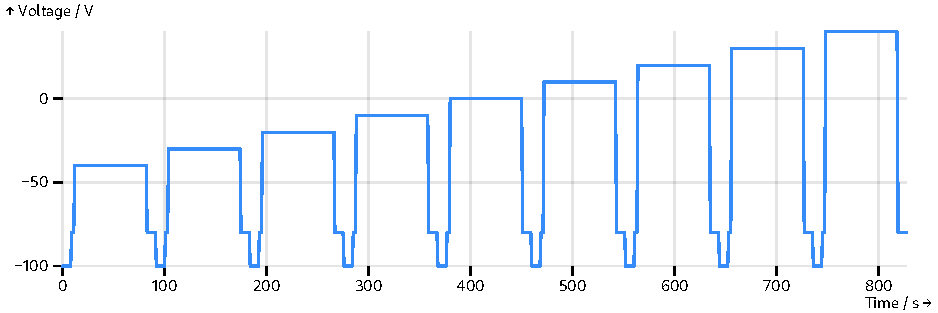
\includegraphics[width=\columnwidth]{../figures/results/voltage-protocol.pdf}
  \caption{The \textit{activation} voltage pulse protocol $V(t)$ used for the measurement and simulation. This is the voltage set across the A549 cell's membrane using a Patch-Clamp-System. The corresponding current is then recorded and depicted in \Cref{figure:full-simulation-current} along with its simulation result.}
  \label{figure:voltage-protocol}
\end{figure}

\section{Results}
\begin{figure}[ht]
  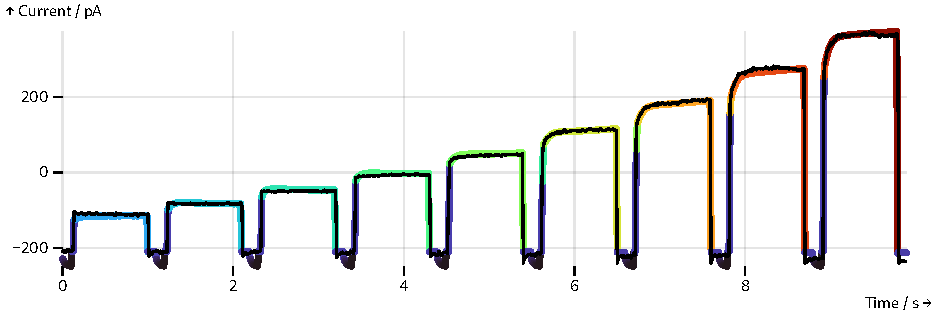
\includegraphics[width=\columnwidth]{../figures/results/full-simulation-current.pdf}
  \caption{The simulated and measured current response $I(t)$ across the membrane of an A549 cancer cell, given the \textit{activation} voltage protocol $V(t)$ in \Cref{figure:voltage-protocol}, recorded in the G0 phase of the cell cycle.}
  \label{figure:full-simulation-current}
\end{figure}
\begin{figure}
  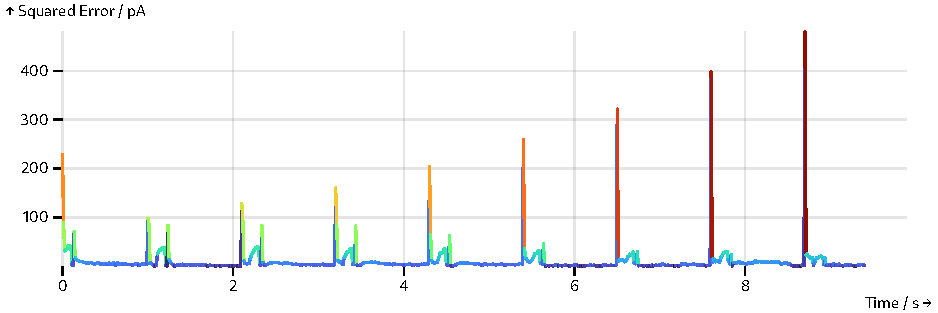
\includegraphics[width=\columnwidth]{../figures/results/simulation-error.pdf}
  \caption{Pointwise squared error between the measured current $\vec{I}_{\rm meas}$ and the simulated current $\vec{I}$, showing potential systematic problems within the computational model's representation of the ion channels as compared to the experimental results.}
  \label{figure:simulation-error}
\end{figure}

\subsection{Adaptive Timestepping}
With the standard forward iteration approach, the simulation takes 412 million steps to simulate over all voltage protocols and cell cycle phases, while the adaptive timestepping only requires 9 million steps for the same configuration.
While keeping the same level of accuracy when matching with the experimental data, our adaptive timestepping method is therefore 45 times faster than the standard approach, on average.

\begin{figure}
  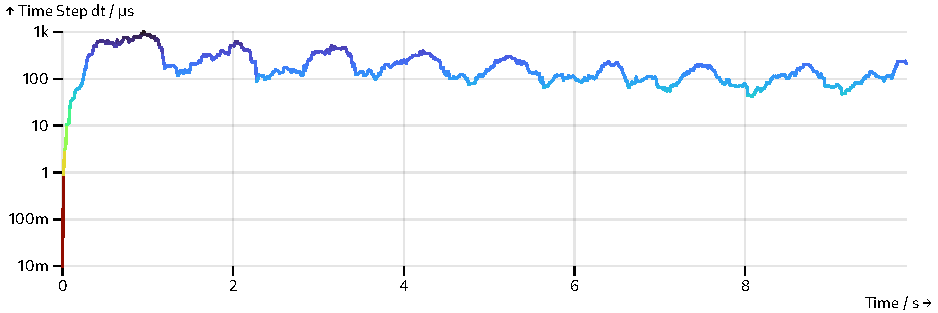
\includegraphics[width=\columnwidth]{../figures/results/dt-plot.pdf}
  \caption{Timestep $\Delta t$ throughout the duration of the simulation. $(\Delta t)_n$ is chosen in between simulation steps based on the heuristic given in \Cref{eq:dt-heuristic}. Red areas (small dt) indicate a high resolution within the simulation, blue areas indicate lower resolution (and therefore higher simulation speed).}
  \label{figure:dt-plot}
\end{figure}

\begin{figure}
  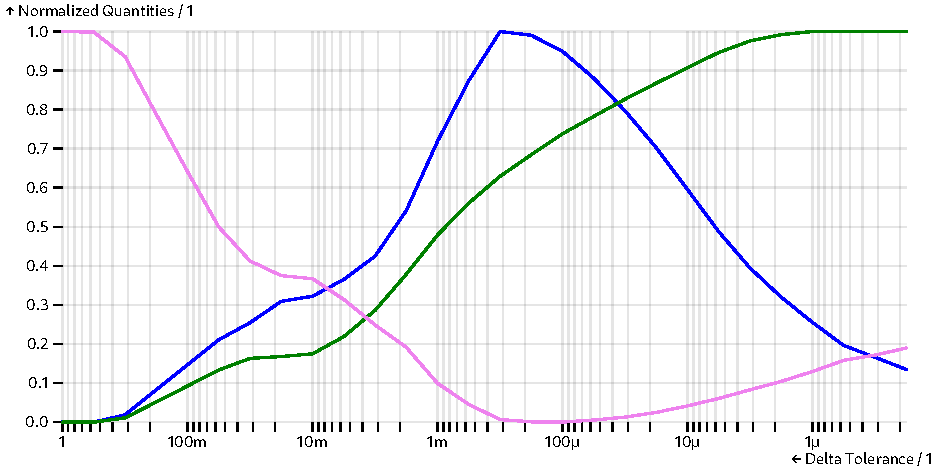
\includegraphics[width=\columnwidth]{../figures/results/delta-tolerance.pdf}
  \caption{Relative change of the average timestep $\Delta t$, simulation runtime and acceptance rate.}
  \label{figure:delta-tolerance}
\end{figure}

\subsection{Inverse Problem}
We compare different optimization approaches based on their runtime and root mean square error,
$$\Delta = \sqrt{\sfrac{1}{N_t} {\textstyle \sum_{j=1}^{N_t}} (I_j - I_{{\rm meas}, j})^2} = \frac{\norm{\vec{I} - \vec{I}_{\rm meas}}}{\sqrt{N_t}}\,.$$

\begin{table}
  \caption{Comparison of Optimization Approaches}
  \begin{tabular}{lll}
    \textbf{Algorithm}                          & \textbf{Runtime} & \textbf{RMSE} \\
    \midrule
    Particle Swarm Optimization                 & 1                & 1             \\
    Non-Negative Least Squares \cite{1997-nnls} & 1                & 1             \\
    Quadratic Program                           & 1                & 1             \\
    Gradient Descent + Penalty                  & 1                & 1             \\
    LBFGS + Penalty                             & 1                & 1             \\
  \end{tabular}
  \label{table:optimization-comparison}
\end{table}

\begin{figure*}[ht]
  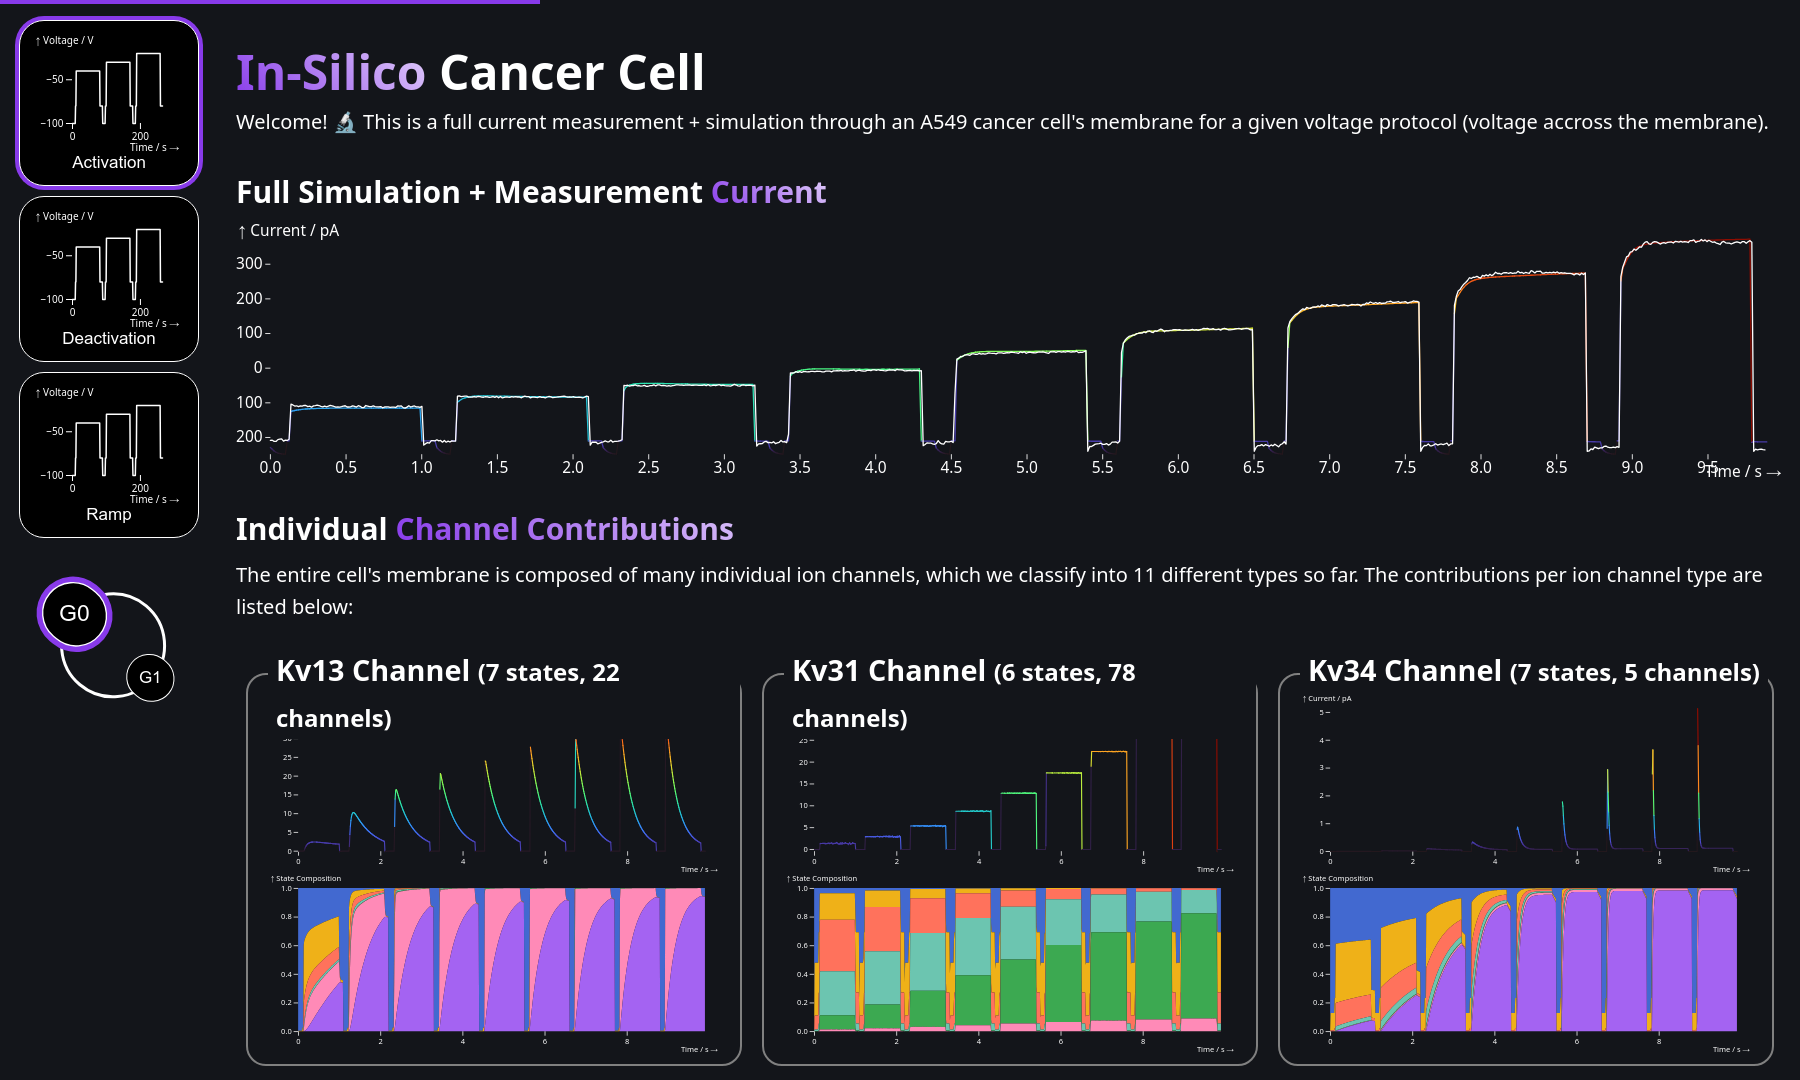
\includegraphics[width=\textwidth]{../figures/above-the-fold-screenshot.png}
  \caption{Screenshot of the live simulation dashboard, available here: \url{https://in-silico-cancer-cell.waldert.at/}. This is the graphical user interface to the simulation written in Rust. The full simulation, completing within around 500ms, runs live in the browser using Rust's bindings to WebAssembly. One can choose the voltage protocol and cell cycle phase (G0/G1) in the menu on the left, while the full current and individual channel currents and internal states can be seen on the right. The remaining ion channel types have been cut off on this screenshot.}
  \label{figure:screenshot}
\end{figure*}

\section{Outlook}
Numerically, the stability of the simulation varies greatly with the time step state change tolerance $\Delta^{\rm tol}$, this could be improved using a higher-order integration scheme.
Regarding the simulation dashboard, there are still many adjustments that could improve and enable further usage perspectives.

  % \pagebreak

  \printbibliography
  % \printnoidxglossary[type=acronym, title={Acronyms}]

  \pagebreak
  \twocolumn[
    \section*{Signatures}
    This project was carried out as part of a \href{https://biotechmedgraz.at}{BioTechMed-Graz} \textit{Lab Rotation}. The aim of the programme is to give interested graduates a chance to broaden their scientific interests beyond the topic of their master's thesis.

    \vspace{4.5cm}
    \SignatureAndDate{(Peter Waldert)}

    \vspace{3cm}
    \SignatureAndDate{(Prof. Christian Baumgartner)}
  ]

  % \pagebreak
  % \appendix
  % \section{Appendix}
\end{document}
